\section{The Rodin Platform}
\label{reference_01}

This Chapter should give the user an overview about the UI elements he might encounter.

\subsection{Eclipse in General}

Just references to other resources.

\subsection{The Event-B Perspective}

\marginpar{The Event-B perspective: We briefly describe the various views (Event-B explorer, structure editor, outline view, symbol view) and their content. We want to cover every element of each view (like buttons, entry fields, etc.), but for the underlying theory we link to the other reference sections. The relevant menu entries are also described.}

Figure \ref{fig_ref_01_eventb_perspective1} shows an overview of the initial situation of the Event-B Perspective. The following subsections name the different Rodin GUI elements (i.e. Views) which are visible and explain their functions.

\imagedpi{img/reference/ref_01_eventb_perspective1.pdf}{150mm}{img/reference/ref_01_eventb_perspective1.png}{Overview of the Event-B Perspective}{fig_ref_01_eventb_perspective1}

\subsubsection{Menu bar}

The menu bar of provides for instance file and edit operations.

\subsubsection{Tool bar}

The tool bar provides short cuts for familiar commands like save, print, undo and redo. Furthermore, the tool bar provides wizard short cuts for creating elements like axioms, constants, enumerated sets, etc. which are described in section \ref{ref_01_the_eventb_editor}.

\subsubsection{Editor View}

The editor view contains the active Event-B editor which is described in section \ref{ref_01_the_eventb_editor}.

\subsubsection{Outline View}

The outline view displays the outline of the active Event-B editor, and lists elements like axioms, variables, etc.. 

\subsubsection{Rodin Problems View}

he Rodin Problems view shows problems (i.e. syntax errors) of the active Event-B editor.

\subsubsection{Symbols View}
\label{reference_01_symbols_view}

The symbols view is intended to give users a convenient way to type in mathematical symbols into the various model editors. If an editor is open and a text field is active (the cursor is blinking), then clicking a symbol inserts it at the current position as demonstrated in figure \ref{fig_ref_01_symbol_table1}. 

The ASCII code corresponding to the symbol where the mouse hovers is also displayed as a tooltip, so that the user can also learn how to input symbols directly. 

\begin{figure}[!h]
\begin{center}
	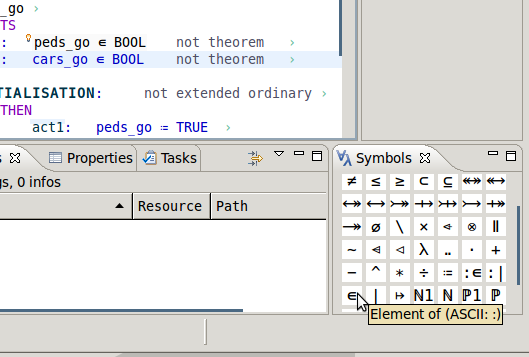
\includegraphics{img/reference/ref_01_symbol_table1.png}
	\caption{Clicking a symbol inserts it at the current position}
	\label{fig_ref_01_symbol_table1}
\end{center}
\end{figure}

\subsubsection{Event-B Explorer}
\label{reference_01_eventb_explorer}

Projects are reachable in the RODIN platform by means of a view called the \textsf{Event-B Explorer}. This view is usually situated on the left hand side of the screen as shown in figure \ref{fig_ref_01_eventb_perspective1}. The \textsf{Event-B Explorer} contains a list of name of the current projects. Next to each project name is a little triangle. By pressing it, one can expand a project and see its components like machines and contexts.

The icons (\icon{rodin/ctx_obj.png} or \icon{rodin/mch_obj.png}) situated next to the components help recognizing their kind (context or machine respectively).

In expanding a machine (respectively a context), you can explore its elements. Double clicking on a specific element (i.e. a variable) opens the Event-B editor and marks the position of the variable in the machine (respectively in the context) as shown in figure \ref{fig_ref_01_project_explorer1}. Furthermore, proof obligations are displayed at tree structure's leafs (for more information see section \ref{ref_01_proving_perspective}).

\begin{figure}[!h]
\begin{center}
	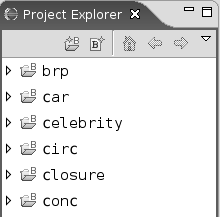
\includegraphics{img/reference/ref_01_project_explorer1.png}
	\caption{Double clicking on an element opens the Event-B editor and marks the corresponding position}
	\label{fig_ref_01_project_explorer1}
\end{center}
\end{figure}

\subsection{The Event-B Editor}
\label{ref_01_the_eventb_editor}

Once a context (or respectively a machine) is created, a window appears in the editing area as shown in figure \ref{fig_ref_01_eventb_editor1}.

\begin{figure}[!h]
\begin{center}
	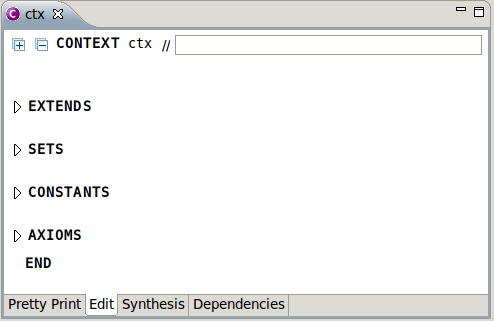
\includegraphics{img/reference/ref_01_eventb_editor1.png}
	\caption{The Event-B editor}
	\label{fig_ref_01_eventb_editor1}
\end{center}
\end{figure}

You are in the "Edit" area allowing you to edit modelling elements of the context, namely dependencies (keyword "EXTENDS"), carrier sets (keyword "SETS"), constants (keyword "CONSTANTS"), or axioms (keyword "AXIOMS"). By pressing the triangle (\icon{rodin/collapsed.png}) next to each keyword, you can add, remove, or move corresponding modelling elements. As an example, figure \ref{fig_ref_01_eventb_editor2} shows what you obtain after pressing the triangle next to the keyword "AXIOMS".

\begin{figure}[!h]
\begin{center}
	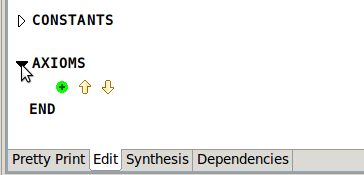
\includegraphics{img/reference/ref_01_eventb_editor2.png}
	\caption{By pressing the triangle you can collapse/expand context sections}
	\label{fig_ref_01_eventb_editor2}
\end{center}
\end{figure}

By pressing the \icon{rodin/add.png} button, you can add a new modelling element. For instance clicking on the \icon{rodin/add.png} button next in the "AXIOMS" section will add a new axiom element. You can now enter a new axiom and a comment in the corresponding boxes as indicated in figure \ref{fig_ref_01_eventb_editor3}.

\begin{figure}[!h]
\begin{center}
	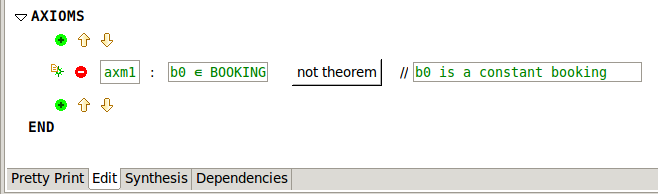
\includegraphics{img/reference/ref_01_eventb_editor3.png}
	\caption{Adding a new modelling element}
	\label{fig_ref_01_eventb_editor3}
\end{center}
\end{figure}

For removing a modelling element, press the \icon{rodin/remove.png} button. You can also move an modelling element up or down by selecting it and then pressing one of the two arrows (\icon{rodin/up_edit.png} or \icon{rodin/down_edit.png}).

It is also possible to add modelling elements by using wizards. You can active the different wizard by using the buttons in the tool bar as shown in figure \ref{fig_ref_01_eventb_editor12} and in figure \ref{fig_ref_01_eventb_editor13} respectively (The wizards depend on the active file machine or context). The next sections explain how to use these wizards.

\begin{figure}[!h]
\begin{center}
	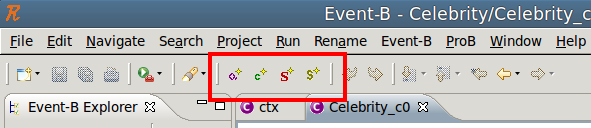
\includegraphics{img/reference/ref_01_eventb_editor12.png}
	\caption{Wizards for context specific elements located in the tool bar}
	\label{fig_ref_01_eventb_editor12}
\end{center}
\end{figure}

\begin{figure}[!h]
\begin{center}
	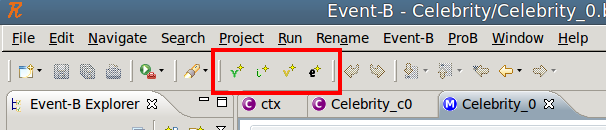
\includegraphics{img/reference/ref_01_eventb_editor13.png}
	\caption{Wizards for machine specific elements located in the tool bar}
	\label{fig_ref_01_eventb_editor13}
\end{center}
\end{figure}


\subsubsection{New Carrier Sets Wizard}

In order to activate the \textsf{New Carrier Sets Wizard}, you have to press the \icon{rodin/newset_edit.png} button located in the tool bar. Pressing the button bring up the window shown in figure \ref{fig_ref_01_eventb_editor4}.

\begin{figure}[!h]
\begin{center}
	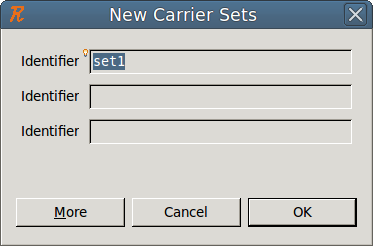
\includegraphics{img/reference/ref_01_eventb_editor4.png}
	\caption{New Carrier Sets Wizard}
	\label{fig_ref_01_eventb_editor4}
\end{center}
\end{figure}

You can enter as many carrier sets as you want by pressing the \textsf{More} button. When you’re finished, press the \textsf{OK} button. 

\subsubsection{New Enumerated Set Wizard}

In order to activate the \textsf{New Enumerated Set Wizard}, you have to press the \icon{rodin/newenuset_edit.png} button located in the tool bar. Pressing the button bring up the window shown in figure \ref{fig_ref_01_eventb_editor5}.

\begin{figure}[!h]
\begin{center}
	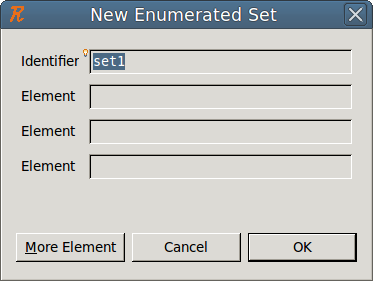
\includegraphics{img/reference/ref_01_eventb_editor5.png}
	\caption{New Enumerated Set Wizard}
	\label{fig_ref_01_eventb_editor5}
\end{center}
\end{figure}

You can enter the name of the new enumerated set as well as the name of its elements. By pressing the \textsf{More Elements} button, you can enter additional elements. When you’re finished, press the \textsf{OK} button. The benefit of using this wizard is for instance when you add the new carrier set \texttt{COLOR} and the three constants \texttt{red}, \texttt{green}, and \texttt{orange} the wizard creates automatically beside the set and constants the following axiom $partition(COLOR , \{red\}, \{green\}, \{orange\})$.

\subsubsection{New Constants Wizard}

In order to activate the \textsf{New Constants Wizard}, you have to press the \icon{rodin/newcst_edit.png} button located in the tool bar. Pressing the button bring up the window shown in figure \ref{fig_ref_01_eventb_editor6}.

\begin{figure}[!h]
\begin{center}
	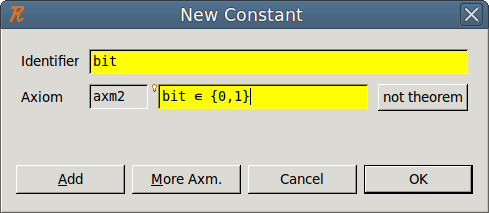
\includegraphics{img/reference/ref_01_eventb_editor6.png}
	\caption{New Constants Wizard}
	\label{fig_ref_01_eventb_editor6}
\end{center}
\end{figure}

You can then enter the names of the constants, and an axiom which can be used to define its type. By pressing \textsf{More Axm.} button you can enter additional axioms. For adding more constants, press the \textsf{Add} button. When you’re finished, press the \textsf{OK} button.

\subsubsection{New Axioms Wizard}

In order to activate the \textsf{New Axioms Wizard}, you have to press the \icon{rodin/newaxm_edit.png} button located in the tool bar. Pressing the button bring up the window shown in figure \ref{fig_ref_01_eventb_editor7}.

\begin{figure}[!h]
\begin{center}
	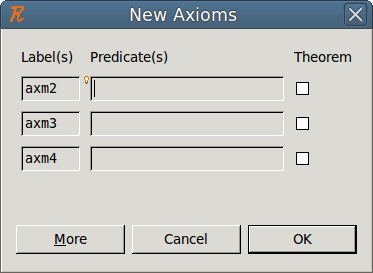
\includegraphics{img/reference/ref_01_eventb_editor7.png}
	\caption{New Axioms Wizard}
	\label{fig_ref_01_eventb_editor7}
\end{center}
\end{figure}

You can then enter the axioms you want. If more axioms are needed then press \textsf{More} button. When you are finished, press \textsf{OK} button.

The "Theorem" checkbox indicates whether the corresponding axiom is a theorem.

\subsubsection{New Variable Wizard}

In order to activate the \textsf{New Variable Wizard}, you have to press the \icon{rodin/newvar_edit.png} button located in the tool bar. Pressing the button bring up the window shown in figure \ref{fig_ref_01_eventb_editor15}.

\begin{figure}[!h]
\begin{center}
	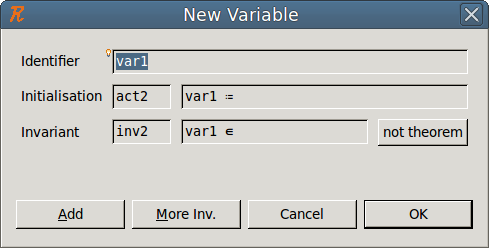
\includegraphics{img/reference/ref_01_eventb_editor14.png}
	\caption{New Variable Wizard}
	\label{fig_ref_01_eventb_editor14}
\end{center}
\end{figure}

You can then enter the names of the variables, its initialization, and an invariant which can be used to define its type. By pressing button \textsf{More Inv.} you can enter additional invariants. For adding more variables, press the \textsf{Add} button. When you’re finished, press the \textsf{OK} button. 

\subsubsection{New Invariants Wizard}

In order to activate the \textsf{New Invariants Wizard}, you have to press the \icon{rodin/newinv_edit.png} button located in the tool bar. Pressing the button bring up the window shown in figure \ref{fig_ref_01_eventb_editor15}.

\begin{figure}[!h]
\begin{center}
	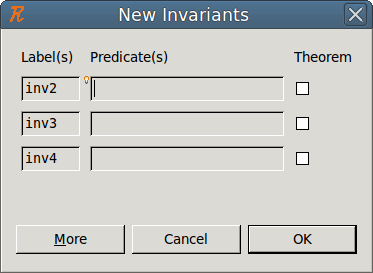
\includegraphics{img/reference/ref_01_eventb_editor15.png}
	\caption{New Invariants Wizard}
	\label{fig_ref_01_eventb_editor15}
\end{center}
\end{figure}

You can then enter the invariants you want. If more invariants are needed then press \textsf{More} button. The \textsf{Theorem} checkbox indicates whether the corresponding invariant is a theorem.

\subsubsection{New Event Wizard}

In order to activate the \textsf{New Events Wizard}, you have to press the \icon{rodin/newevt_edit.png} button located in the tool bar. Pressing the button bring up the window shown in figure \ref{fig_ref_01_eventb_editor16}.

\begin{figure}[!h]
\begin{center}
	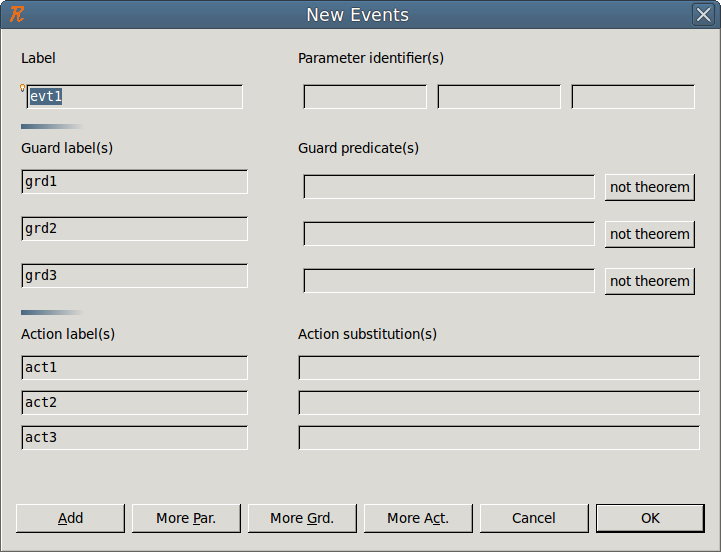
\includegraphics{img/reference/ref_01_eventb_editor16.png}
	\caption{New Event Wizard}
	\label{fig_ref_01_eventb_editor16}
\end{center}
\end{figure}

You can then enter the events you want. As indicated, the following elements can be entered: name, parameters, guards, and actions. More parameters, guards and actions can be entered by pressing the corresponding buttons. If more events are needed then press the \textsf{Add} button. Press the \textsf{OK} button when you’re finished.

Note that an event with no guard is considered to have a true guard. Moreover, an event with no action is considered to have the "skip" action. 

\subsubsection{Dependencies (Context)}

By selecting the "Dependencies" tab of the editor, you obtain the window as shown in figure \ref{}.

\begin{figure}[!h]
\begin{center}
	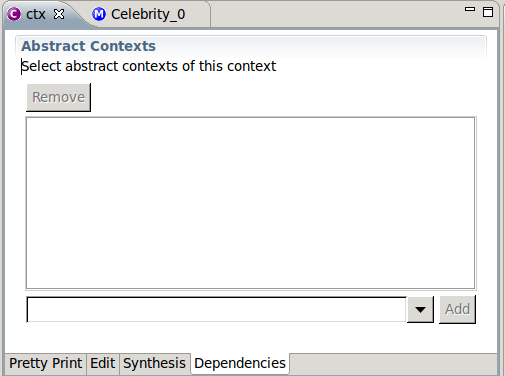
\includegraphics{img/reference/ref_01_eventb_editor8.png}
	\caption{Dependencies tab of the Event-B editor}
	\label{fig_ref_01_eventb_editor8}
\end{center}
\end{figure}

The dependencies tab allows you to express that the current context is extending other contexts of the current project. In order to add the name of the context you want to extend, use the combobox which appears at the bottom of the window and then select the corresponding context name.

There exists another way to directly create a new context extending an existing one. Select the context in the project window, then press the right mouse key, you’ll get the following menu and select \textsf{Extend}. This should bring up the window as shown in figure \ref{fig_ref_01_eventb_editor9}.

\begin{figure}[!h]
\begin{center}
	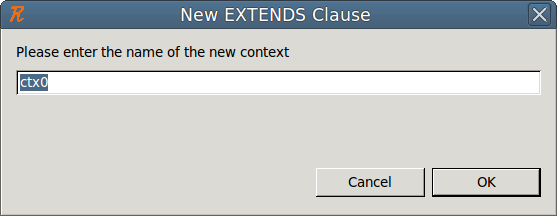
\includegraphics{img/reference/ref_01_eventb_editor9.png}
	\caption{New EXTENDS Clause window}
	\label{fig_ref_01_eventb_editor9}
\end{center}
\end{figure}

You can then enter the name of the new context which will be made automatically an extension of your chosen context. 

\subsubsection{Dependencies (Machine)}

The "Dependencies" tab of machines is very similar to the one of contexts expect of that two kinds of dependencies can be established: machine dependency in the upper part and context dependencies in the lower part.

\subsubsection{Synthesis (Context)}

By selecting the "Synthesis" tab, you may have a global view of your context's elements (carrier set / constant / axiom / extended context) as demonstrated in figure \ref{fig_ref_01_eventb_editor11}. 

\begin{figure}[!h]
\begin{center}
	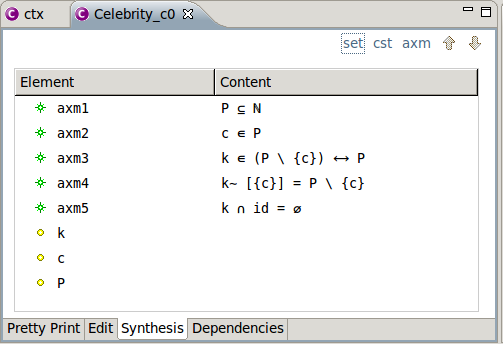
\includegraphics{img/reference/ref_01_eventb_editor11.png}
	\caption{The Synthesis tab of the Event-B editor}
	\label{fig_ref_01_eventb_editor11}
\end{center}
\end{figure}

After pressing set (respectively cst or axm), you can filter carrier sets of your context (respectively constants or axioms).

If you select for example an axiom, you can change its priority order by pressing \icon{rodin/up_edit.png} or \icon{rodin/down_edit.png}‎. You can do the same for carrier sets, constants or extended contexts.

After a right click in this view a contextual menu will pop up which allows you to add new carrier sets, constants, axioms or a new extended context. 

\subsubsection{Synthesis (Machine)}

The "Systhesis" tab of machines is very similar to the one of contexts except of that you may have a global view of your machine's elements (refined machine/seen context/variable/invariant/event/variant).

\subsubsection{Pretty Print}

By selecting the "Pretty Print" tab, you may have a global view of your context as if it would have been entered through an input text file as demonstrated in figure \ref{fig_ref_01_eventb_editor10}.

\begin{figure}[!h]
\begin{center}
	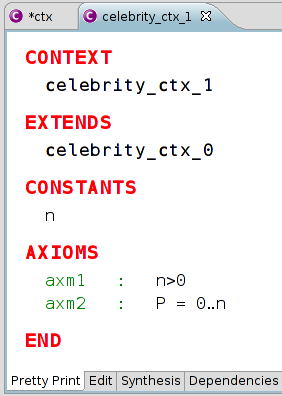
\includegraphics{img/reference/ref_01_eventb_editor10.png}
	\caption{The Pretty Print tab of the Event-B editor}
	\label{fig_ref_01_eventb_editor10}
\end{center}
\end{figure}

\subsection{The Proving Perspective}
\label{ref_01_proving_perspective}

When proof obligations (POs) (\ref{proof_obligation}) are not discharged automatically the user can attempt to discharge them interactively using the Proving Perspective. This page provides an overview of the Proving Perspective and its use. If the Proving Perspective is not visible as a tab on the top right-hand corner of the main interface, the user can switch to it via \textsf{Window $\rangle$ Open Perspective}.

The Proving Perspective consists of a number of views: the \textsf{Proof Tree}, the \textsf{Goal}, the \textsf{Selected Hypotheses}, the \textsf{Proof Control}, the \textsf{Search Hypotheses}, the \textsf{Cache Hypotheses} and the \textsf{Proof Information}. In the discussion that follows we look at each of these views individually. Figure \ref{fig_ref_01_proving_perspective1} shows an overview of the Proving Perspective.

\imagedpi{img/reference/ref_01_proving_perspective1.pdf}{150mm}{img/reference/ref_01_proving_perspective1.png}{Overview of the Proving Perspective}{fig_ref_01_proving_perspective1}

\subsubsection{Loading a Proof}

To work on an undischarged PO it is necessary to load the proof into the Proving Perspective. To do this switch to the Proving Perspective; select the project from the Event-B Explorer; select and expand the component (context or machine); and finally select (double-click) the proof obligation of interest. A number of views will be updated with details of the corresponding proof. 

Note that pressing \icon{rodin/discharged.png} button on the top left hand side of the \textsf{Event-B Explorer} will remove all discharged proof obligations (PO's) from the view. 

\subsubsection{The Proof Tree}

The proof tree view provides a graphical representation of each individual proof step, as seen in figure \ref{fig_ref_01_proving_perspective2}.

\begin{figure}[!h]
\begin{center}
	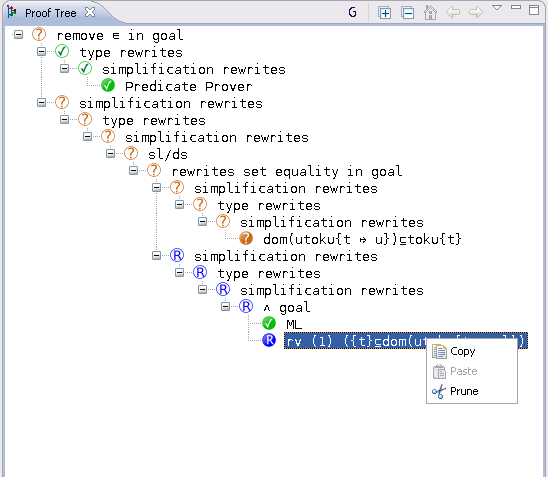
\includegraphics{img/reference/ref_01_proving_perspective2.png}
	\caption{The Proof Tree}
	\label{fig_ref_01_proving_perspective2}
\end{center}
\end{figure}

Each node in the tree corresponds to a sequent. A line is right shifted when the corresponding node is a direct descendant of the node of the previous line. Each node is labeled with a comment which indicates which rule has been applied, or which prover discharged the proof. By selecting a node in the proof tree, the corresponding sequent is loaded: the hypotheses of the sequent are loaded to the \textsf{Selected Hypotheses window}, and the goal of the sequent is loaded to the \textsf{Goal view}.

The leaves of the tree are decorated with one of three icons:

\begin{itemize}
	\item \icon{rodin/discharged.png} means that this leaf is discharged,
	\item \icon{rodin/pending.png} means that this leaf is not discharged,
	\item \icon{rodin/reviewed.png} means that this leaf has been reviewed. 
\end{itemize}

Internal nodes in the proof tree are decorated in reverse colours. Note that a "reviewed" leaf is one that is not discharged yet by the prover. Instead, it has been "seen" by the user who decided to postpone the proof. Marking nodes as "reviewed" is very convenient since the provers will ignore these leaves and focus on specific areas of interest. This allows interactive proof in a gradual fashion. In order to discharge a "reviewed" node, select it and prune the tree at that node: the node will become "brown" again (undischarged) and you can now try to discharge it. 

On top of the proof tree view, one can see three buttons:

\begin{itemize}
	\item \icon{rodin/showgoal.png} buttons allows you to see the goal of the sequent corresponding to each node,
	\item \icon{rodin/collapseall.png} button allows you to fully expand the proof tree,
	\item \icon{rodin/expandall.png} allows you to fully collapse the tree: only the root stays visible. 
\end{itemize}

The little square (with a "+" or "-" inside) next to each node in the proof tree allows you to expand or collapse the subtree starting at that node. 

The proof tree can be pruned at a selected node; the subtree of the selected node is removed from the proof tree. The selected node becomes a leaf and is decorated with \icon{rodin/pending.png}. The proof activity can then be resumed from this node. After selecting a node in the proof tree pruning can be performed in two ways:

\begin{itemize}
	\item by right-clicking and then selecting "Prune",
	\item by clicking on the \icon{rodin/pn_prover.png} button in the proof control view. 
\end{itemize}

Note that after pruning, the post-tactic is not applied to the new current sequent. The post-tactic should be applied manually, if required, by clicking on the post-tactic button in the Proof Control view. This is useful, in particular, when you want to redo a proof from the beginning. The proof tree can be pruned at its root node and then the proof can proceed again, with invocation of internal or external provers; or with interactive proof.

Before pruning a particular node, the node (and its subtree) can be copied to the clipboard. If the new proof strategy subsequently fails, the copied version can be pasted back into the pruned node (see the next section). 

By selecting a node in the proof tree and then right-clicking with the mouse, you can copy the part of the proof tree starting at that sequent (the node and its subtree). Pasting the node and subtree back in is done in a similar manner, with a right mouse click on a proof node. This allows reuse of part of a proof tree in the same, or even in another, proof.

\subsubsection{Goal and Selected Hypotheses}

The nodes in the proof tree view correspond to sequents. A user will work with one selected node, and thus one sequent, at a time; attempting various strategies in an effort to show that the sequent goal is true. The \textsf{Goal} and \textsf{Selected Hypotheses} views provide information to the user about the currently selected sequent. Figure \ref{fig_ref_01_proving_perspective3} shows an example.

\begin{figure}[!h]
\begin{center}
	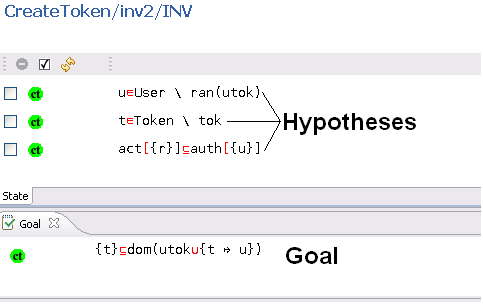
\includegraphics{img/reference/ref_01_proving_perspective3.png}
	\caption{Open proof obligation}
	\label{fig_ref_01_proving_perspective3}
\end{center}
\end{figure}

A hypothesis can be removed from the list of selected hypotheses by selecting the check the box situated next to it (you can click on several boxes) and then by clicking on the \icon{rodin/remove.png} button at the top of the selected hypotheses window.

Note that the deselected hypotheses are not lost: you can find them again using the \textsf{Search Hypotheses} \icon{rodin/sh_prover.png} button in the Proof Control view. Other buttons are used as follows:

\begin{itemize}
	\item \icon{rodin/select_all_prover.png} select all hypotheses. 
	\item \icon{rodin/inv_prover.png} invert the selection. 
	\item \icon{rodin/falsify_prover.png} next to the goal - proof by contradiction 1: The negation of the goal becomes a selected hypothesis and the goal becomes "$\bot$". 
	\item \icon{rodin/falsify_prover.png} next to a selected hypothesis - proof by contradiction 2: The negation of the hypothesis becomes the goal and the negated goal becomes a selected hypothesis. 
\end{itemize}

A user wishing to attempt an interactive proof has a number of proof rules available, and these may be either rewrite rules or inference rules. In the \textsf{Goal} and the \textsf{Selected Hypotheses} views various operators may appear in red coloured font. The red font indicates that some interactive proof rule(s) are applicable and may be applied as a step in the proof attempt. When the mouse hovers over such an operator a number of applicable rules may be displayed; the user may choose to apply one of the rules by clicking on it. Figure \ref{fig_ref_01_proving_perspective4} shows an example.

Other proof rules can be applied when green buttons appear in the \textsf{Goal} and \textsf{Selected Hypotheses} views. Examples are proof by contradiction \icon{rodin/falsify_prover.png}, that we have already encountered; and \icon{rodin/conjI_prover.png} for conjunction introduction in the goal. 

\begin{figure}[!h]
\begin{center}
	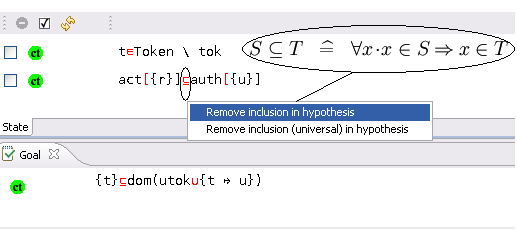
\includegraphics{img/reference/ref_01_proving_perspective4.png}
	\caption{Applying a rule}
	\label{fig_ref_01_proving_perspective4}
\end{center}
\end{figure}

To instantiate a quantifier the user enters the desired expression in the box behind the quantifier and clicks on the quantifier as demonstrated in figure \ref{fig_ref_01_proving_perspective5}.

\begin{figure}[!h]
\begin{center}
	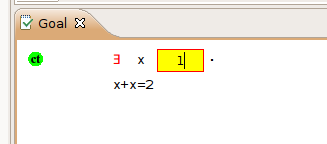
\includegraphics{img/reference/ref_01_proving_perspective5.png}
	\caption{Instantiating a quatifier}
	\label{fig_ref_01_proving_perspective5}
\end{center}
\end{figure}

\subsubsection{The Proof Control View}

The \textsf{Proof Control view} contains the buttons which you can use to perform an interactive proof. 

\begin{figure}[!h]
\begin{center}
	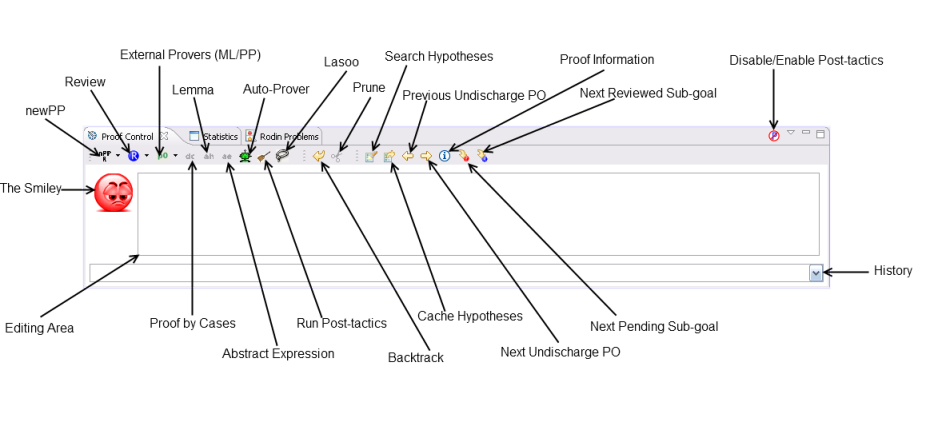
\includegraphics{img/reference/ref_01_proving_perspective6.png}
	\caption{The Proof Control View}
	\label{fig_ref_01_proving_perspective6}
\end{center}
\end{figure}

The Proof Control view offers a number of buttons whose effects we briefly describe next; moving from left to right on the toolbar:

\begin{itemize}
    \item \icon{rodin/nppr.png} invokes the new predicate prover, a drop-down list indicates alternative strategies.
    \item \icon{rodin/reviewed.png} indicates that a node has been reviewed: in an attempt by the user to carry out proofs in a stepwise fashion, they might decide to postpone the task of discharging some proofs until a later stage. To do this the proofs can be marked as reviewed by choosing the proof node and clicking on this button. This indicates that by visually checking the proof the user is convinced that they can discharge it later, but they do not want to do it right now.
    \item (p0) the PP and ML provers can be invoked from the drop-down list using different forces.
    \item \icon{rodin/dc_prover.png} do proof by cases: the proof is split into two branches. In the first branch:- the predicate supplied by the user is added to the Selected Hypotheses, and the user attempts to discharge this branch. In the second branch :- the predicate supplied by the user is negated and added to the Selected Hypotheses; the user then attempts to discharge this branch. 
    \item \icon{rodin/ah_prover.png} add a new lemma: the predicate in the editing area should be proved by the user. It is then added as a new selected hypothesis.
    \item \icon{rodin/ae_prover.png} abstract expression: the expression in the editing area is given a fresh name.
    \item \icon{rodin/auto_prover.png} invokes the auto-prover which attempts to discharge the goal. The auto-prover is applied automatically on all proof obligations after a "save" without any intervention of the user. Using this button, you can invoke the auto-prover within an interactive proof.
    \item \icon{rodin/broom_prover.png} executes the post-tactics,
    \item \icon{rodin/lasoo_prover.png} load into the Selected Hypotheses window those hidden hypotheses that contain identifiers in common with the goal, and with the selected hypotheses.
    \item \icon{rodin/bk_prover.png} backtracks form the current node (i.e., prune its parent),
    \item \icon{rodin/pn_prover.png} prune the proof tree from the node selected in the proof tree,
    \item \icon{rodin/sh_prover.png} find hypotheses containing the character string in the editing area, and display in the Search Hypothesis view.
    \item \icon{rodin/ch_prover.png} press this to display the "Cache Hypotheses" view. This view displays all hypotheses that are related to the current goal.
    \item \icon{rodin/prev_prover.png} loads the previous undischarged proof obligation,
    \item \icon{rodin/next_prover.png} loads the next undischarged proof obligation,
    \item \icon{rodin/info_prover.png} show information corresponding to the current proof obligation in the corresponding window. This information correspond to the elements that directly took part in the proof obligation generation (events, invariant, etc.),
    \item \icon{rodin/next_pd.png} goto the next pending node of the current proof tree,
    \item \icon{rodin/next_rv.png} load the next reviewed node of the current proof tree.
\end{itemize}

Furthermore, you can disable/enable post-tactics which allows you to choose whether post-tactics run after each interactive proof step. In addition you can open the preferences for post-tactics. For this, open the menu of the \textsf{Proof Control View} via the little triangle on the top right corner of the view.

The smiley can be one of three different colors: (1) red, indicates that the proof tree contains one or more undischarged sequents, (2) blue, indicates that all undischarged sequents of the proof tree have been reviewed, (3) green, indicates that all sequents of the proof tree are discharged.

The editing area allows the user to supply parameters for proof commands. For example, when the user attempts to add a new hypothesis (by clicking on the lemma ah button), the new hypothesis should have been written by the user in the editing area.

ML (mono-lemma) prover appears in the drop-down list under the button (pp) as M0, M1, M2, M3, ML. The different configuration (e.g., M0) refer to the proof force of the ML prover. All hypotheses are passed to ML.

PP (predicate prover) appears in the drop-down list under the button (pp) as P0, P1, PP.

\begin{itemize}
	\item P0 uses all selected hypotheses (the ones in Selected Hypotheses window).
	\item P1 employs a lasoo operation to the selected hypotheses and the goal, and uses the resulting hypotheses.
	\item PP uses all hypotheses. 
\end{itemize}

\subsubsection{The Search Hypotheses View}

By typing a string in the Proof Control window and pressing the Search Hypotheses button a window is provided which contains the hypotheses having a character string in common with the one entered by the user in the editing area. For example, if we search for hypotheses involving the character string "cr", then after pressing the Search Hypothesis button on the proof control window, we obtain the following: 

---------------------------------------------------------------------------------------------------------------------

If we type 'inv' in the filter area, we'll obtain the following:

\begin{figure}[!h]
\begin{center}
	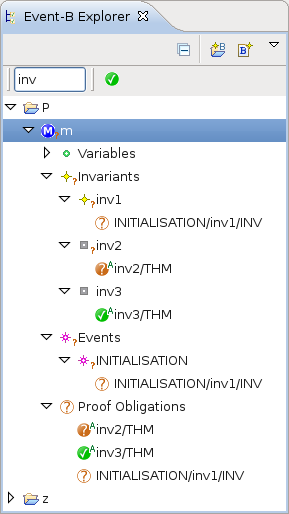
\includegraphics{img/reference/ref_01_project_explorer5.png}
	\caption{Project Explorer View with expanded project}
	\label{fig_ref_01_project_explorer5}
\end{center}
\end{figure}

This is exactly the same, nothing was filtered out because all PO names contain 'inv' as substring. Now, if we add '2', we will only have POs related to invariant 'inv2', as follows: 

\begin{figure}[!h]
\begin{center}
	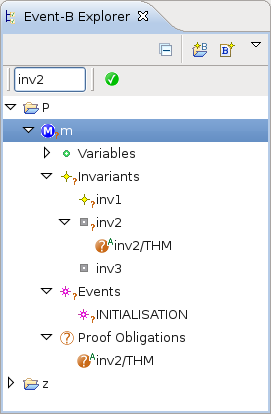
\includegraphics{img/reference/ref_01_project_explorer6.png}
	\caption{Project Explorer View with expanded project}
	\label{fig_ref_01_project_explorer6}
\end{center}
\end{figure}

Now, let's see what we obtain if we type in 'THM': 

\begin{figure}[!h]
\begin{center}
	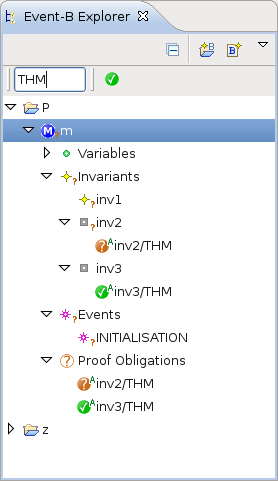
\includegraphics{img/reference/ref_01_project_explorer7.png}
	\caption{Project Explorer View with expanded project}
	\label{fig_ref_01_project_explorer7}
\end{center}
\end{figure}

Only theorems are displayed, the entry 'INITIALISATION/inv1/inv' has been filtered out because it contains no 'THM' substring.

Note: filtering is case sensitive, thus 'thm' is different from 'THM'.

Beside the input text box is a green button, the same that is used in the explorer for discharged POs. Clicking this button hides discharged POs: 

\begin{figure}[!h]
\begin{center}
	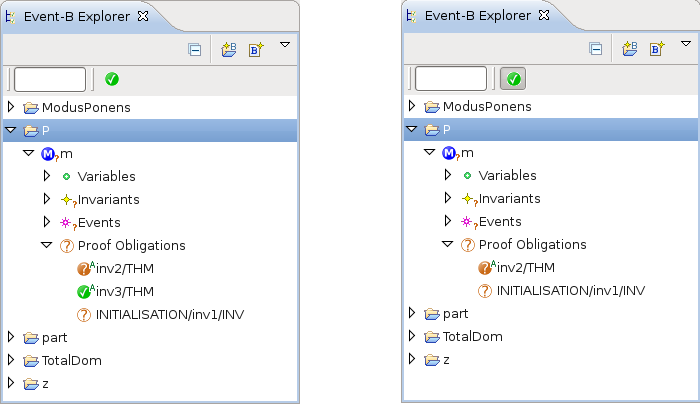
\includegraphics{img/reference/ref_01_project_explorer8.png}
	\caption{Project Explorer View with expanded project}
	\label{fig_ref_01_project_explorer8}
\end{center}
\end{figure}

It's also possible to combine text filter and discharged filter: 

\begin{figure}[!h]
\begin{center}
	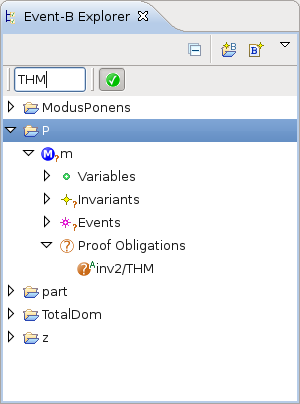
\includegraphics{img/reference/ref_01_project_explorer9.png}
	\caption{Project Explorer View with expanded project}
	\label{fig_ref_01_project_explorer9}
\end{center}
\end{figure}

In the above example, INITIALISATION/inv1/INV is filtered out by the text filter (does not contain 'THM') and inv3/THM is filtered out by the discharged PO filter. 

\subsubsection{Problems View}
\label{reference_01_the_problems_view}

When the Static Checker discovers an error in a project, a little "x" is added to this project and to the faulty component in the "Project Explorer" window as shown in figure \ref{fig_ref_01_problemsview1}.

The error itself is shown by opening the "Problems" window (see figure \ref{fig_ref_01_problemsview2}). 

By double-clicking on the error statement, you are transferred automatically into the place where the error has been detected so that you can correct it easily as shown in figure \ref{fig_ref_01_problemsview3}. 

We do basically the same as for the Event-B perspective. The views are proof tree, goal, control and statistics.
 
\subsection{Preferences}

We briefly describe what preference can be set for Rodin. For their deeper meaning, we'll refer to the other sections (esp. the prover settings).

\subsubsection{Customize Prefixes}

\marginpar{CONTENT MIGRATED FROM WIKI!}

This page describes the mechanism used to set element prefixes, and perform renaming using dedicated actions for both machines and contexts. Note that prefixes are used for automatic renaming when element should be alphanumerically ordered, as well as for new element creation. 

Principles

This mechanism is close to eclipse preferences and properties settings. In our case, the prefixes are in any case, defined globally for a workspace scope. If the user does not set specific settings for prefixes at the workspace scope, the default prefixes which are given by elements contributions are used. Moreover, if the user changes the prefixes once, they will then be persisted. The new feature is here the ability for one to set up some specific settings for prefixes at a project scope. The settings will be then persisted through a file attached to the project settings (i.e., the prefixes used will be shared at export).

Summary

\begin{itemize}
	\item Default prefixes correspond to Rodin's default values,
	\item A user can modify workspace settings via "Window" > "Preferences" menu,
	\item Workspace modifications are persisted from one session to another,
	\item Project specific settings can be set up and will then be persisted in a project scope,
	\item Restoring default prefixes for a project will enable the current workspace prefix settings,
	\item Restoring default prefixes for the workspace will reset the prefixes to their original values corresponding to the values which are set at Rodin's first launch. 
\end{itemize}

Overview 

%\begin{figure}[!h]
%\begin{center}
%	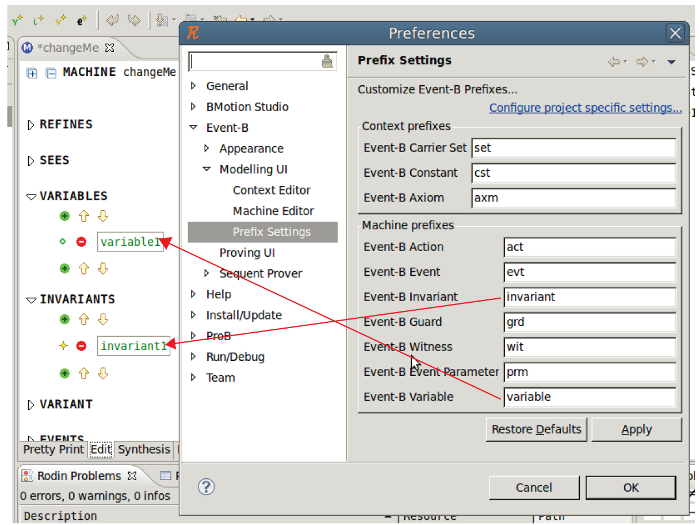
\includegraphics{img/reference/ref_01_preferences1.png}
%	\caption{The Structured Editor}
%	\label{fig_ref_01_preferences1}
%\end{center}
%\end{figure}

The image above shows that modifying prefixes at a workspace scope or project scope, will affect the names used at creation of new Event-B elements. On this image, one can see that the prefix for a variable (resp. invariant) originally set to "var" (resp. "inv") has been replaced by "variable" (resp. "invariant"). New elements are then named using those prefixes.

How to set prefixes

Prefix settings can be accessed through 2 differents ways depending on the scope of their application:

Workspace scope settings

Window > Preferences > Event-B > Modelling UI > Prefix settings, 
    
%\begin{figure}[!h]
%\begin{center}
%	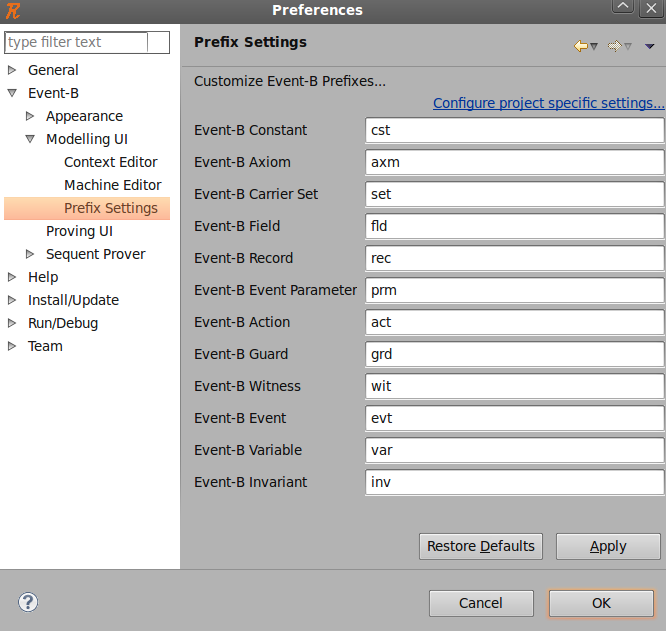
\includegraphics{img/reference/ref_01_preferences2.png}
%	\caption{The Structured Editor}
%	\label{fig_ref_01_preferences2}
%\end{center}
%\end{figure}

or directly via,

    Rename > Customize prefixes... (The rename menu appeared in previous releases as the refactoring menu) 

%\begin{figure}[!h]
%\begin{center}
%	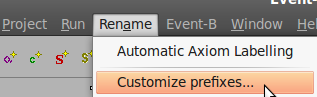
\includegraphics{img/reference/ref_01_preferences3.png}
%	\caption{The Structured Editor}
%	\label{fig_ref_01_preferences3}
%\end{center}
%\end{figure}

Project scope settings

    by right-clicking on a project and then choosing "Properties",
    Menu "Project > Properties",
    or via the Window > Preferences and then click on the link "Configure project specific settings". In this case, one will have to choose the project on which the prefixes should be set up. This is allowed via a specific project selection dialog. After the project selection, a dialog for prefix settings opens for the selected project. 

A dialog (see picture below) appears, where a page handling prefixes settings, allows one user to customize prefixes for a chosen project. One this page, the user can toggle the button "Enable project specific settings".

    If this button is enabled :
        the prefixes used are those which are specified at this project level, 
    If this button is not enabled :
        the prefixes used are those which are defined at a workspace level. 

%\begin{figure}[!h]
%\begin{center}
%	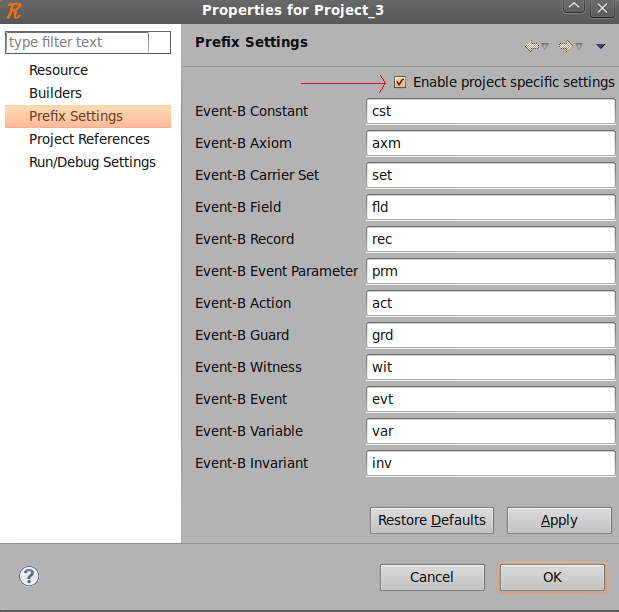
\includegraphics{img/reference/ref_01_preferences4.png}
%	\caption{The Structured Editor}
%	\label{fig_ref_01_preferences4}
%\end{center}
%\end{figure}

Automatic Renaming

    One action is available for Context files.
        Automatic Axiom Labelling : this action will perform alphanumeric renaming on axioms given their order of appearance.
 
%\begin{figure}[!h]
%\begin{center}
%	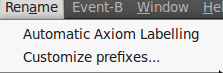
\includegraphics{img/reference/ref_01_preferences5.png}
%	\caption{The Structured Editor}
%	\label{fig_ref_01_preferences5}
%\end{center}
%\end{figure}

Three actions are available for Machine files.

    Automatic Invariant Labelling : this action will perform alphanumeric renaming on invariants given their order of appearance,
    Automatic Guard Labelling : this action will perform alphanumeric renaming on guards given their order of appearance,
    Automatic Action Labelling : this action will perform alphanumeric renaming on guards given their order of appearance. 

%\begin{figure}[!h]
%\begin{center}
%	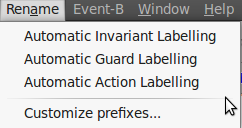
\includegraphics{img/reference/ref_01_preferences6.png}
%	\caption{The Structured Editor}
%	\label{fig_ref_01_preferences6}
%\end{center}
%\end{figure}

\subsubsection{Preferences for the automatic tactics}

\marginpar{CONTENT MIGRATED FROM WIKI!}

\paragraph{Introduction}

The purpose is to give more detailed preferences to the user to build his own automated tactics. More precisely, the user should on the one hand have a way to specify which parameters have to be passed to the reasoners, and on the other hand to construct complex proof strategies.

\paragraph{User Documentation}

Here is the documentation about the current implementation of automatic tactics preferences: Auto-tactic \& Post-tactic

\paragraph{Tactic Combinators}

Tactic combinators can be used to construct complex proof strategies.

Historically, one combinator exists since the beginning of auto tactic preferences: the "loop on all pending". It takes one or more tactics and loops them over every pending child, until all tactic fail. Until Rodin 2.3, it is the only combinator in Rodin; it is used on the configurable list of auto and post tactics. Rodin 2.3 pushes configurability forward, by providing several other combinators and auto tactic editors.

The following is a list of combinators present by default.

One may notice the absence of child-specific combinator, i.e applying tactic T1 on first child, T2 on second child, ..., whereas this kind of combinator exists in other provers. The reason is that we are constructing here auto tactics, that is tactics to be attempted in a general context. In provers with child-specific combinators, they are used to make manual proofs, hence needing proof-specific adaptation.

\subparagraph{Composers}

A composer combinator applies its given tactic(s) to the given node. The given node may be open or closed. It succeeds if at least 1 tactic application succeeded. 

\begin{center}
    \begin{tabular}{ | l | l | l | l | p{5cm} |}
    \hline
	Name & Arity & Description & Stops when  \\ \hline
	Sequence & 1..n  & applies given tactics in given order & all tactics have been applied  \\ \hline
	Compose until Success & 1..n  & applies given tactics in given order & a tactic application succeeds \\ \hline
	Compose until failure  & 1..n  & applies given tactics in given order & a tactic application fails \\ \hline
	Loop & 1 & applies given tactic repeatedly & the child tactic application fails \\ \hline
    \end{tabular}
\end{center}

\subparagraph{Selectors}

A selector combinator applies its given tactic to the set of nodes it selects. Selected nodes are computed from the given node. The given node may be open or closed. It succeeds if the tactic application succeeded for at least 1 selected node. 

\begin{center}
    \begin{tabular}{ | l | l | l | p{5cm} |}
    \hline
	Name & Arity & Selects \\ \hline
	On all pending  & 1 & all pending children of the given node (the given node itself if it is open) \\ \hline
    \end{tabular}
\end{center}

\subparagraph{Post Actions}

A post actions applies its given tactic to the given node. The given node must be open (else it fails). Then, it performs a specific treatment, guarded by a trigger condition. 

\begin{center}
    \begin{tabular}{ | l | l | l | l | p{5cm} |}
    \hline
	Name & Arity & Trigger Condition & Post Action \\ \hline
	Attempt & 1 & the given node still has pending children (subtree not closed) & prune proof tree at given node  \\ \hline
    \end{tabular}
\end{center}

\subparagraph{Loop on All pending}

$loopOnAllPending(T_1 \ldots T_n) \;\;\defi\;\; loop(onAllPending(composeUntilSuccess(T_1 \ldots T_n)))  $

\paragraph{Other Ideas}

    timeout: a post action of arity 1 (with duration as input): limits the time allocated for the tactic it is applied to (fails after time has gone out)

    limitDepth: a post action of arity 1 (with depth as input): limits the proof tree depth for the tactic it is applied to (prevents tree from growing beyond a given depth) 

\subsubsection{Proof Skeleton View}

\marginpar{CONTENT MIGRATED FROM WIKI!}

The text field on top of the \textsf{Event-B Explorer} can be used to filter displayed proof obligations. Only POs with a name that contains the input text will appear in the view. We will start an example from the following: 

To browse through a proof, you can use the Proof Skeleton View.

As can be seen in the screen shot above, machine "celebrity\_1" of project "celebrity" is expanded. We find seven proof obligations. Each of them has got a compound name as indicated in the tables below. A green logo situated on the left of the proof obligation name states that it has been proved (an A means it has been proved automatically). If you switch in proving perspective and click on the proof obligation name in the Event-B Explorer, you are transferred into a window where you can handle your proof. We are going to describe it more precisely in subsequent sections.



Purpose

The Proof Skeleton View allows to quickly browse through a proof built either automatically or interactively with the Rodin prover. This view can be used on any proof, independently of the presence of a corresponding proof obligation.

Furthermore, this view allows user to see together proof rules and corresponding sequents.

The Proof Skeleton View
Showing the View

The Proof Skeleton View is available as other views in the Window > Show View > Other > Event-B > Proof Skeleton View menu.

To watch a proof skeleton, simply select a proof obligation or a proof file in the Event-B Explorer.

View Interpretation

Proof skeletons are displayed in a two-part view. On the left-hand side is the tree structure of rules applied in the proof. On the right-hand side stands the sequent on which the currently selected rule is applied. The proof which is displayed is the one stored in the proof file on disk, never the one which is currently edited through the proof control. This can be very handy as it can allow one to see the previous proof of a proof obligation while working on a new proof of it. 

%\begin{figure}[!h]
%\begin{center}
%	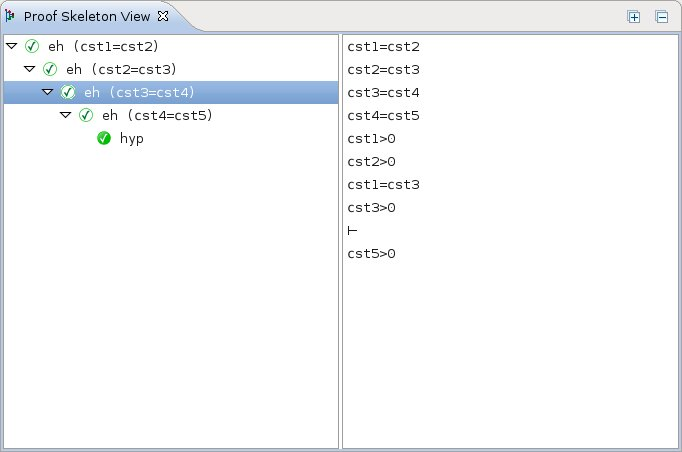
\includegraphics{img/reference/ref_01_proofskeletonview1.jpg}
%	\caption{A typical example of machine and context relationship}
%	\label{fig_ref_01_proofskeletonview1}
%\end{center}
%\end{figure}

The tree can be expanded or collapsed by using [+] and [-] buttons on the upper right corner.

Copy/Paste to Proof Tree

The copy/paste feature allows to reuse a stored proof into a new proof. Starting from the following configuration: 

%\begin{figure}[!h]
%\begin{center}
%	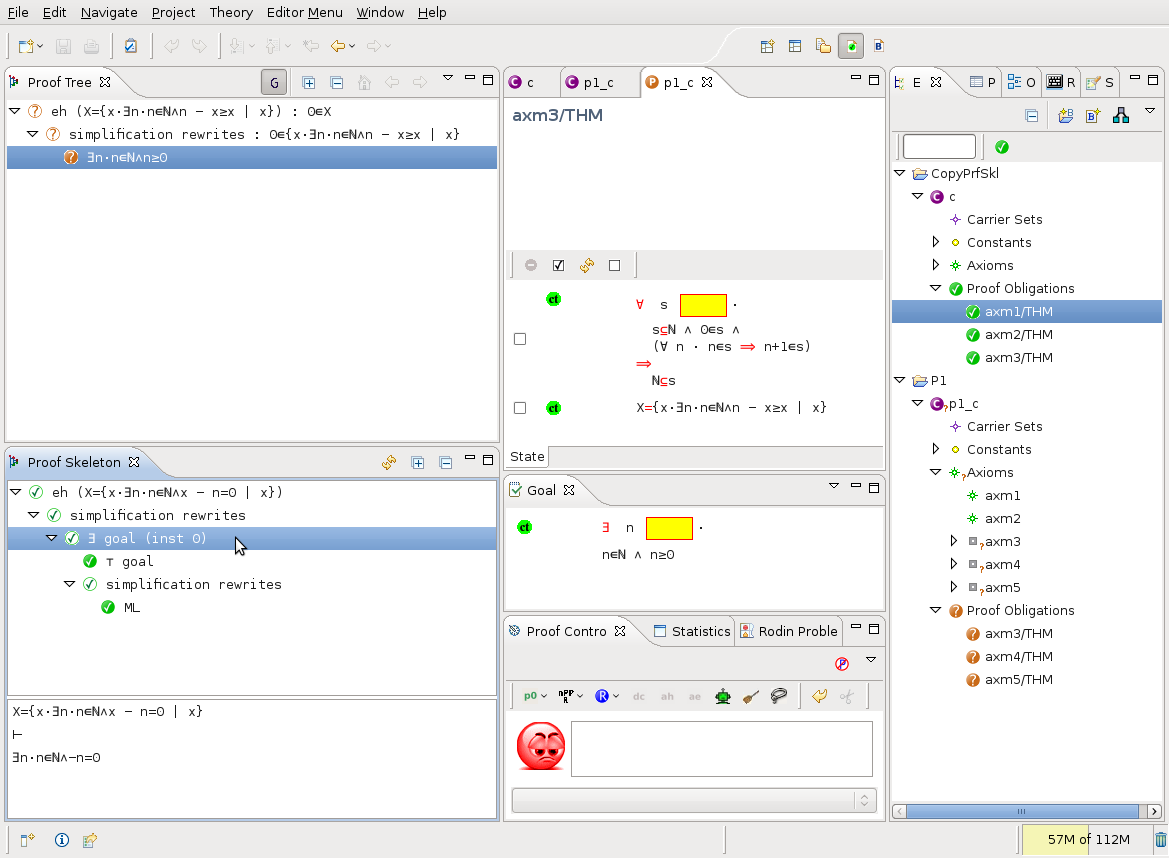
\includegraphics{img/reference/ref_01_proofskeletonview2.png}
%	\caption{A typical example of machine and context relationship}
%	\label{fig_ref_01_proofskeletonview2}
%\end{center}
%\end{figure}

where the proof we are working on (top left) is similar to another proof whose skeleton is displayed on bottom left. We can then copy/paste the interesting sub tree from the skeleton to the proof: 

%\begin{figure}[!h]
%\begin{center}
%	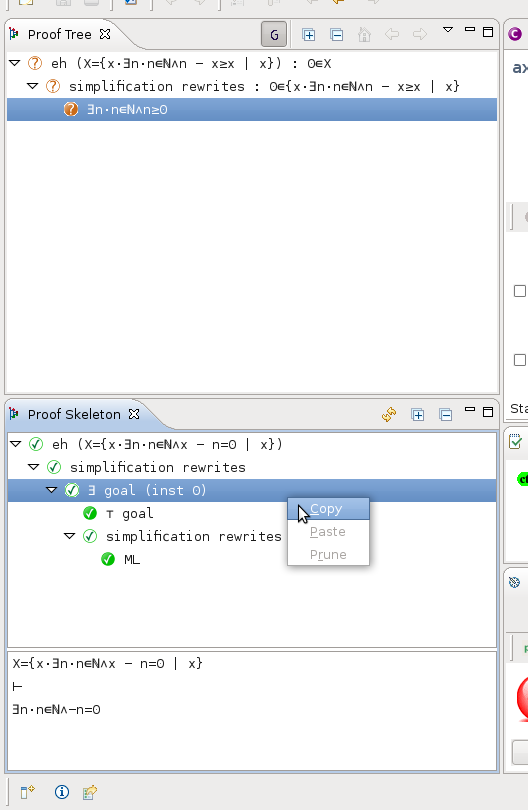
\includegraphics{img/reference/ref_01_proofskeletonview3.png}
%	\caption{A typical example of machine and context relationship}
%	\label{fig_ref_01_proofskeletonview3}
%\end{center}
%\end{figure}

%\begin{figure}[!h]
%\begin{center}
%	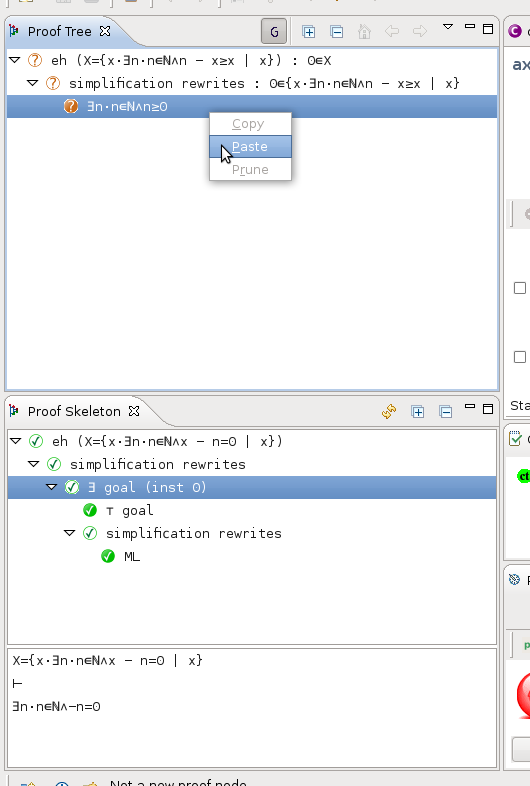
\includegraphics{img/reference/ref_01_proofskeletonview4.png}
%	\caption{A typical example of machine and context relationship}
%	\label{fig_ref_01_proofskeletonview5}
%\end{center}
%\end{figure}

%\begin{figure}[!h]
%\begin{center}
%	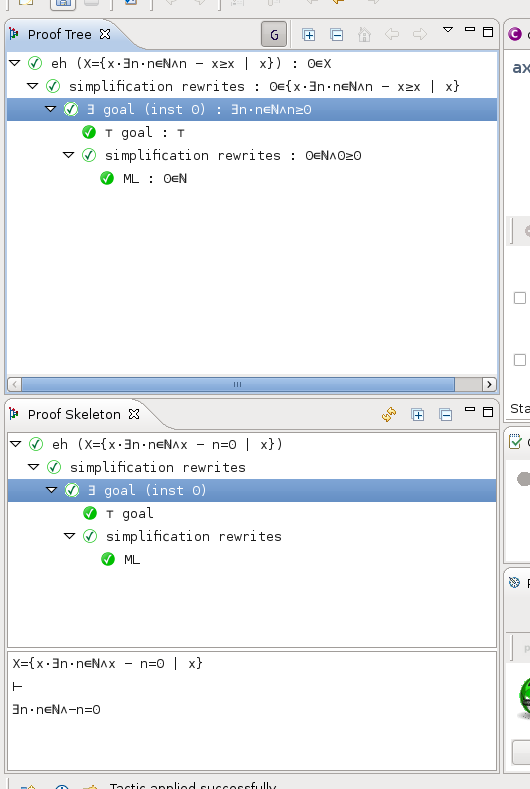
\includegraphics{img/reference/ref_01_proofskeletonview5.png}
%	\caption{A typical example of machine and context relationship}
%	\label{fig_ref_01_proofskeletonview5}
%\end{center}
%\end{figure}

